\documentclass{sig-alternate}

\setcopyright{acmcopyright}
\usepackage{amsmath}
\usepackage{amssymb}
\usepackage{framed}
\usepackage{url}
%\usepackage[disable]{todonotes}
\usepackage{todonotes}
\usepackage{graphicx}
\usepackage{float}
\usepackage{tabularx}
\usepackage{fancyvrb}

\begin{document}

\title{Nipping Bugs in the Bud\\ Student Mistakes in Introductory Computer Science}
\numberofauthors{3}
\author{
\alignauthor
%Nivedita Chopra\\
%       \affaddr{Carnegie Mellon University}\\
%      \affaddr{Pittsburgh, PA}\\
%     \email{niveditc@andrew.cmu.edu}
%     \additionalauthors{Additional authors: Robert Simmons (Carnegie Mellon University,
%email: {\texttt{rjsimmon@cs.cmu.edu}}) and Roy Maxion
%(Carnegie Mellon University, email: {\texttt{maxion@cs.cmu.edu}}).}
}
%\date{\today}
\maketitle

\presetkeys{todonotes}{color=red!30}{}
% TODO : Remove page numbers before submission
\setcounter{page}{1}
\pagenumbering{arabic}

% IEEE bug counts
\def\numlogicIEEE{66 }
\def\numdataIEEE{24 }
\def\numinterfaceIEEE{7 }
\def\numotherIEEE{26 }

% Final bug counts
\def\numlogic{63 }
\def\numdata{21 }
\def\numinterface{7 }
\def\numcomp{32 }
\def\numtotal{123 }
\def\numedge{31 }

\begin{abstract}
Bugs in computer programs may be caused by mistakes in the programmer's thought process. Mitigating the causes of common mistakes in introductory computer science classes can help improve the quality of code that students write in future classes, as well as in industry or academia. We want to mitigate common mistakes made by students in our class by analyzing the bugs committed by students in the class, determining the mistakes in thought processes that caused these bugs, and devising ways to correct these mistakes by changing our teaching methods. We collected information about bugs committed by students, including a description of the bug, an optional code snippet, and the student's reasoning behind the bug. We then classified each bug according to a standard taxonomy (IEEE Standard Classification of Software Anomalies (2010)), determined the mistakes behind common bugs, and proposed ways to mitigate such mistakes. We found \numlogic logic bugs, \numdata data bugs, and \numinterface interface bugs per the IEEE standard. An additional category of bugs emerged that we called ``comprehension errors'' (\numcomp instances), which is unique to introductory computer science classes. Comprehension errors are caused by a misunderstanding of concepts, specifications, or error messages, and may prove useful in highlighting concepts that need to be explained better.

\end{abstract}

\section{Introduction}
\label{sec:intro}

Bugs are a major problem in software development, and bugs in software that is widely used can have far-reaching consequences, as was recently seen in the case of the Heartbleed bug in OpenSSL. While slips in syntax can be detected and fixed easily, oftentimes bugs are caused by mistakes in the programmer's thought process. For example, a student who has misunderstood the workings of pointer arithmetic may add the wrong quantity to a pointer, causing memory errors. Such mistakes ought to be detected and remedied early on, preferably in introductory and intermediate programming classes, to ensure that the programmers of tomorrow are much less likely to commit certain kinds of errors.

\section{Problem and Approach}
Many mistakes that students make during the course of an introductory computer science course may not be corrected before the end of the semester. Thus students continue to make these mistakes, which may lead to them writing buggy code in higher-level classes and/or industry, where there is no longer a focus on basic computer science concepts.\\

Our approach is to catalog the bugs committed by students in an introductory computer science class. By analyzing these bugs, we hope to gain insight into mistakes in students' thought processes. Based on our analysis, we will devise ways to mitigate these mistakes, such as changing our method of instruction, or changing the way that students think about bugs or about the problems they are solving.

\section{Background and related work}
\label{sec:background}

In the 1980s, much research was aimed at examining bugs committed by students learning to program, and determining flaws in student reasoning from a cognitive standpoint \cite{JoniSolowayGoldmanEhrlich83, PutnamSleemanBaxterKuspa86, SpohrerSoloway86, Pea86}. Much of this work was focused on the student's understanding of specific language constructs such as loops, conditional statements, arrays, etc. \cite{JoniSolowayGoldmanEhrlich83, PutnamSleemanBaxterKuspa86, Pea86}. An example illustrating this is a student misunderstanding of the semantics of a while loop, and making the assumption that the loop condition is being checked at every point within the loop body and not just at the beginning of each iteration of the loop \cite{Pea86}.\\

Most of the work done in the 1980s focused on novice programmers who were learning to program for the first time \cite{SpohrerSoloway86, Pea86}. Our research focuses on students who already know how to program, having taken at least one semester-long programming class. Thus we focus on the students' understanding of algorithms and data structures, and other concepts they are learning for the first time. We also classify the bugs committed by students in the class in a broader sense and avoid focusing on details that are specific to our class and the language in which it is taught (C0 and C).\\

%\todo[inline]{Got rid of Ko and Myers paragraph. Hope it transitions okay.}
%Ko and Myers' work \cite{KoMyers03} classifies and describes errors in programming by linking the errors to their causes. Their model for programming errors is based on Reason's model \cite{Reason90}. Reason's model demonstrates that mistakes in applying knowledge and strategy cause the cognitive problems that lead to errors. Ko and Myers provide a broad taxonomy for errors seen in all types of programming, including both industry and education. Ko and Myers share our goal of connecting errors in programming to mistakes in the programmer's thought process. However, our research focuses on introductory programming classes, and we provide a taxonomy tailored for that purpose.\\

Recently, some research has been done in introductory computer science classes to examine the problems that students face in these classes with an aim of alleviating student frustration and attrition \cite{BryceCooleyHansenHayrapetyan10}. They follow a similar method to ours, of asking students to fill in a form reporting their bugs, yet they differ from our research in two important aspects. Firstly, their classification of bugs is very detailed, with 20 disjoint categories, and focuses heavily on particular concepts and ideas covered in the class, so it is not applicable beyond their class without changes. Additionally, they do not examine student reasoning behind the bug, and classify bugs entirely based on the description and code for the bug.\\

For the purposes of our research, it is important to distinguish between bugs, which are errors based on flawed knowledge, and slips, which are errors based on ``random noise'' \cite{VanLehn90}. While programming, slips are usually manifested as syntax errors and some other errors that may cause a program to fail compilation. On the other hand, bugs are caused by mistakes in the programmer's thought process. In our research, we consider only bugs and we ignore slips entirely. This is because slips in programming are self-correcting, since they almost always cause compile errors which can be easily fixed by the programmer.\\

Our research was performed in an introductory computer science class --- Principles of Imperative Computation (15-122) at Carnegie Mellon University. This class is taught in C0, which is a small safe subset of the C programming language, augmented with contracts \cite{Arnold10, PfenningCortinaLovas11}, and in C. The class introduces computer science students to basic algorithms such as searching and sorting, data structures such as lists, stacks, queues, heaps, trees, etc. and computational ideas such as complexity analysis and proof of correctness of code.


\section{Method}
\label{sec:method}

We recorded bugs committed by the students in Principles of Imperative Computation (15-122) in Fall 2014. Each record of data contained a description of the bug, an optional snippet of the buggy code, and a short explanation by the student of the cause behind the committing of the bug. An example of a record of data is shown in Figure \ref{fig:record}.\\

\begin{figure}
\begin{framed}
\emph{What was the bug?}\\
\verb|NULL| pointer dereference\\

\emph{What caused you to write buggy code?}\\
 I did not think of edge cases while writing the code\\

\emph{Include a snippet of the buggy code (optional)}\\
\verb|list = list->next;| //where \verb|list| is \verb|NULL|
\end{framed}
\caption{Example of a record of data}
\label{fig:record}
\end{figure}


Bugs were obtained and recorded in the following ways:
\begin{itemize}
\item{\textbf{Google form.} Students were asked to fill an online form when they found and fixed a bug. In addition to the data points mentioned above, data from this source also contained information on how much time it took the student to find and fix their bug, how they found the bug, and suggestions for how the course staff may have done better in this regard.} %A screenshot of the form we used is included in Figure \ref{fig:form}}.

%\begin{figure*}
%\centering
%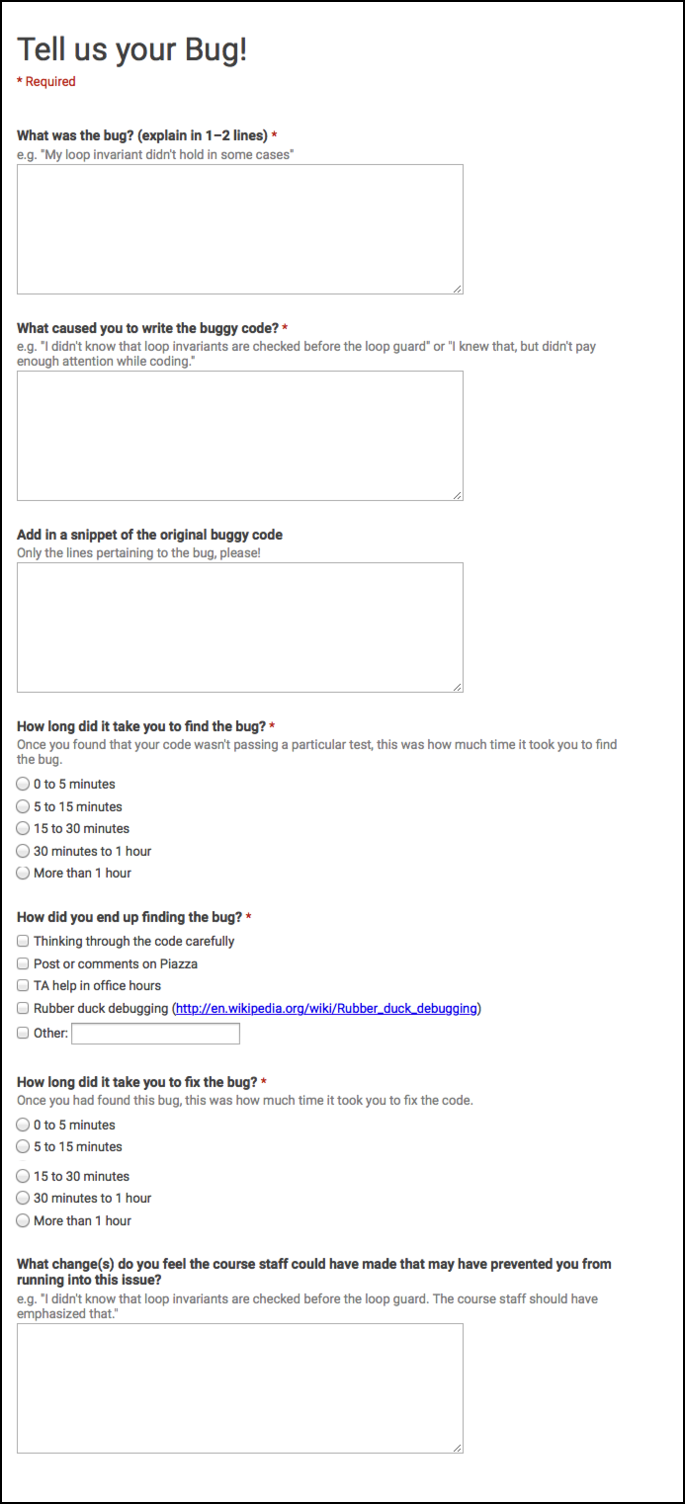
\includegraphics[scale=0.41]{figures/form.png}
%\caption{Snapshot of the online Google form that was used to collect data}
%\label{fig:form}
%\end{figure*}
% DONE : Include a snapshot of the form in a figure

\item{\textbf{Student observation.} We observed students in labs and office hours and took note of the bugs committed by students in those settings. In this setting, when students fixed their bugs, usually with our help, we asked them to explain their bug and their reasoning behind what caused them to commit the bug.}
\item{\textbf{Piazza.} We analyzed posts made in the online Q\&A forum, Piazza, and recorded the bugs seen there. These posts included a description and/or code pertaining to the bug, and a discussion that led to the bug being solved. We only recorded bugs in which the discussion included student comments that illustrated their reasoning behind the bug.}
\end{itemize}

\begin{table*}
\def\arraystretch{1.75}
\centering
\caption{Error classification by type as per the IEEE Standard Classification for Software Anomalies \cite{IEEE10}}
\label{table:IEEE}
\begin{tabular}{|p{1in}|p{3in}|p{2.4in}|} \hline
\textbf{Type} & \textbf{Description} & \textbf{Example}\\ \hline
Data Error&
Defect in data definition, initialization, mapping, access or use as found in a model, specification or implementation.&
Failure to initialize a variable, modifying data structures during non-destructive operations, dereferencing null, etc.\\ \hline

Logic Error&
Defect in decision logic, branching, sequencing, or computational algorithm, as found in natural language specifications or in
implementation language.&
Incorrect sequencing of code statements, missing cases, performing the wrong operation, etc.\\ \hline

Interface Error&
Defect in specification or implementation of an interface (e.g., between user and machine, between two internal software modules, between software module and database, between internal and external software components, between software and hardware, etc.)&
Use of implementation functions in client code, writing an implementation that does not conform to the interface, etc.\\ \hline

Syntax Error&
Nonconformity with the defined rules of a language.&
Missing semicolon, mismatched parentheses, etc.\\ \hline

Description Error&
Defect in description of software or its use, installation, or operation.&
\\ \hline

Standards Error&
Nonconformity with a defined standard.&
\\ \hline

Other Error&
Defect with no defined type.
&
\\ \hline
\end{tabular}
\end{table*}


With a view towards further examining these bugs, we classified them according to the IEEE Standard Classification for Software Anomalies \cite{IEEE10}. This document provides a standard for classifying anomalies seen during software development. It enables organizations to get insight into the bugs seen during their software development process \cite{IEEE10}.\\

The IEEE standard classifies software anomalies seen in production code on the basis of attributes such as status, priority, severity, probability, effect, type, mode, and insertion activity \cite{IEEE10}. For the purposes of our research, we only care about the classification based on type, as outlined in Table \ref{table:IEEE}.\\


When we classified the collected bugs according to the IEEE standard, we noticed that bugs fell into the logic error (\numlogicIEEE instances), data error (\numdataIEEE instances) and interface error (\numinterfaceIEEE instances) categories. \numotherIEEE instances were categorized as other errors, with no defined type. Three logic errors and three data errors were later reclassified as comprehension bugs (Section \ref{sec:comprehension}).\\

None of our bugs fell into the other three categories of the IEEE standard --- syntax error, description error and standards error. As explained in Section \ref{sec:background}, syntax errors are slips by the programmer, and not bugs, hence they do not appear in our taxonomy of bugs. We do not encounter description errors as we operate under the assumption that the specification provided to students does not contain errors, since it has been thoroughly playtested by the course staff. Additionally, we do not deal with standards, hence standard error is irrelevant.\\

By examining the reasoning provided by students, we realized that we could classify all the bugs that fell into the ``other'' error category of the IEEE standard as ``comprehension errors,'' which are described in the next section.

\section{Comprehension Errors}
\label{sec:comprehension}

While classifying bugs seen in our research, we developed a new category of bugs that is not described by the IEEE classification. We call this new category ``comprehension errors,'' and we feel that it may be unique to introductory computer science classes. A comprehension error occurs when the bug seen is caused due to a misunderstanding on the student's part. Comprehension errors can be roughly divided into four types.
\vspace{0.06in}

\subsection{Using the wrong algorithm or paradigm}
\label{sec:comp1}
Often when a task is described to students, they are unsure about which paradigm or algorithm to use to accomplish it. They may misunderstand the use cases of certain algorithms and paradigms and attempt to solve the problem using an inappropriate algorithm. Figure \ref{fig:comp1} illustrates a comprehension error that involves the use of the wrong algorithm.

\begin{figure}
\begin{framed}
\setlength{\parindent}{0cm}
\textbf{Problem} \\
Find the index of the number \texttt{x} in a given array \texttt{A} containing unique numbers, and return -1 if \texttt{x} is not in \texttt{A}.\\

\textbf{Buggy solution} \\
Use binary search to find \texttt{x} in \texttt{A}.\\

\textbf{Correct solution}\\
Use linear search to find \texttt{x} in \texttt{A}.\\

\textbf{Comprehension error}\\
Binary search cannot be used here since the array is not necessarily sorted. This indicates a lack of understanding of the use case for binary search. We assume that the student correctly understood the specifications.
\end{framed}
\caption{Comprehension error due to using the wrong algorithm or paradigm}
\label{fig:comp1}
\end{figure}

\subsection{Misunderstanding specifications}
\label{sec:comp2}
Students are often unfamiliar with reading specifications, and are hence likely to misunderstand them and to make incorrect assumptions while programming. They may also not understand how to use functions that are provided to help them with generating test cases for their code. Figure \ref{fig:comp2} illustrates a comprehension error that is caused by a misunderstanding of the specifications.\\

The bug illustrated in Figure \ref{fig:comp1} could have been caused by a student's incorrect assumption that the input array is always sorted. If this were the case, the bug in Figure \ref{fig:comp1} would be a comprehension error due to misunderstanding specifications rather than due to using the wrong algorithm or paradigm, as explained in Section \ref{sec:comp1}. In situations like this, we must examine student reasoning behind the bug to determine the correct cause of the bug.

\begin{figure}
\begin{framed}
\setlength{\parindent}{0cm}
\textbf{Problem}
Create the list containing 1, 2, and 4, in order, using the \texttt{cons} and \texttt{nil} functions.\\
\texttt{list cons(int, list); /* Adds the integer to the beginning of the list */\\ list nil(); /* Creates a new empty list */}\\

\textbf{Buggy solution}\\
\texttt{list L = cons(1, cons(2, cons(4)));}\\

\textbf{Correct solution}\\
\texttt{list L = cons(1, cons(2, cons(4, nil())));}\\

\textbf{Comprehension error}\\
Misunderstanding the specification of \texttt{cons} and \texttt{nil}.
\end{framed}
\caption{Comprehension error due to misunderstanding specifications}
\label{fig:comp2}
\end{figure}

\subsection{Misunderstanding error messages}
Due to having limited prior programming experience and possibly because they are using new tools, students are often stumped by error messages and warnings, both from the compiler and from Autolab which autogrades submitted code. Figure \ref{fig:comp3} illustrates a comprehension error that is caused by the misunderstanding of an error message.

\begin{figure}
\begin{framed}
\setlength{\parindent}{0cm}
\textbf{Problem} \\
Perform the bitwise AND operation on two integers \texttt{x} and \texttt{y}.\\

\textbf{Buggy solution} \\
\verb|int z  = x && y|\\

\textbf{Error message}\\
\texttt{:error: type mismatch expected bool found int}\\

\textbf{Correct solution}\\
\verb|int z = x & y|\\

\textbf{Comprehension error}\\
Upon reading the error message, the student thinks that \texttt{x} and \texttt{y} should be booleans rather than integers, because they fail to realize that this error message can also indicate problem with the operator rather than the operands.
\end{framed}
\caption{Comprehension error due to misunderstanding error messages}
\label{fig:comp3}
\end{figure}

\subsection{Lacking clarity on a concept}
When learning a computer science concept, such as integer casting or pointer arithmetic, students may not fully understand the concept, leading them to use these ideas incorrectly while attempting to solve a problem. Figure \ref{fig:comp4} illustrates a comprehension error caused by lack of clarity on a concept.

\begin{figure}
\begin{framed}
\setlength{\parindent}{0cm}

\textbf{Problem}\\
Compute the offset as a signed 16 bit integer that is given as a two-byte operand	to the instruction. Instructions are stored in an array of (unsigned) bytes (\verb|ubyte *P|) \\

\textbf{Buggy solution}
\begin{verbatim}
 int16_t o1 = (int16_t)(int8_t)P[pc+1];
 int16_t o2 = (int16_t)(int8_t)P[pc+2];
 int16_t offset = ((o1 << 8) | o2);
\end{verbatim}

\textbf{Correct solution}
\begin{verbatim}
 int16_t o1 = (int16_t)(int8_t)P[pc+1];
 int16_t o2 = (int16_t)(uint16_t)P[pc+2];
 int16_t offset = ((o1 << 8) | o2);
\end{verbatim}

\textbf{Comprehension error}\\
Casts both \verb|o1| and \verb|o2| into signed integers to make resultant offset signed. Sign extension on \verb|o2| may alter the final quantity. This shows a misunderstanding of the concept of sign extension.

\end{framed}
\caption{Comprehension error due to lack of clarity on a concept}
\label{fig:comp4}
\end{figure}


\section{Analysis}
\label{sec:analysis}

The bugs observed were logic bugs (\numlogic instances), data bugs (\numdata instances), and interface bugs (\numinterface instances), as per the IEEE Standard Classification for Software Anomalies. An additional category of bugs, with \numcomp observed instances, emerged here that was not specified in the IEEE classification. These are what we have called ``comprehension errors'' (Section \ref{sec:comprehension}).\\

For the bugs that were frequently observed every week, we sought the student misconceptions that may have led to that bug. Since we possessed a timestamp for each bug recorded, we could pinpoint the context in which the bug was made, based on the material covered and assignments due around that time. The reasoning provided by the students, as described in our data collection process in Section \ref{sec:method}, often gave us an insight into the misconception that caused them to write that bug. In other cases, we employed the method of ``just-so stories,'' \cite{JoniSolowayGoldmanEhrlich83} which tries to reconstruct the thought process that may have led to a particular bug, and provides a convincing hypothesis about the student misconception that led to a particular bug. It is worth highlighting the dangers of using the ``just-so'' method to determine student misconceptions from their code. As discussed in Section \ref{sec:comp2}, the comprehension bug illustrated in Figure \ref{fig:comp1} can be categorized as using the wrong algorithm (Section \ref{sec:comp1}) or as misunderstanding the specification (Section \ref{sec:comp2}).\\

%Each week, we noted the common misconceptions and used these as a basis for modifying some course material for the subsequent semester. \\

% TODO : Add descriptions to table

\begin{table*}
\def\arraystretch{1.75}
\centering
\caption{Proposed Bug Taxonomy}
\label{table:new-taxonomy}
\begin{tabular}{|p{0.95in}|p{1.6in}|p{2in}|p{2.1in}|} \hline
Type&Example : Instructions&Example : Buggy Code&Example : Correct Code\\ \hline
Logic Bug
%\emph{Defect in decision logic, branching, sequencing, or computational algorithm, as found in natural language specifications or in implementation language.}
&
Traverse through a linked list performing a certain	operation on each element
&
\begin{verbatim}
while (li->next != NULL){
 //do something;
 li = li->next;
}
\end{verbatim}
&
\begin{verbatim}
while (li != NULL){
 //do something;
 li = li->next;
}
\end{verbatim}\\
\hline
Data Bug
%\emph{Defect in data definition, initialization, mapping, access or use as found in a model, specification or implementation.}
&
Write a function to check if a given integer is in a linked list
&
\begin{verbatim}
bool is_in(list L, int n){
 while(L->start != NULL){
  if(L->start->data == n)
   return true;
  L->start =
           L->start->next;
 }
 return false;
}
\end{verbatim}
&
\begin{verbatim}
bool is_in(list L, int n){
 list temp = L->start;
 while(temp != NULL){
  if(temp->data == n)
   return true;
  temp = temp->next;
 }
 return false;
}
\end{verbatim}\\
\hline
Interface Bug &
Write a function that removes the green component of a given pixel
\vspace{0.11in}

\emph{Interface}
\vspace{-0.11in}
\begin{verbatim}
pixel make_pixel(
  int a, int r,
  int g, int b);
int get_red(pixel p);
\end{verbatim}

\emph{Implementation}
\verb|typedef int pixel;|
&
\begin{verbatim}
pixel remove_red(pixel p){
   return (p & 0xFF0000);
}
\end{verbatim}
&
\begin{verbatim}
pixel remove_red(pixel p){
   int a = get_alpha(p);
   int g = get_green(p);
   int b = get_blue(p);
   return
    make_pixel(a, 0, g, b);
}
\end{verbatim}\\
\hline
Comprehension Bug &
Create the list containing 1, 2, and 4, in order, using the cons and nil functions

\verb|list cons(int, list);|
\verb|list nil();|
&
\begin{verbatim}
list L =
  cons(1, cons(2,
              cons(4)));
\end{verbatim}
&
\begin{verbatim}
list L =
  cons(1, cons(2, cons(4,
                  nil())));
\end{verbatim}
\\ \hline
\end{tabular}
\end{table*}

Based on our analysis, we propose a new taxonomy of bugs that occur in introductory computer science classes. This taxonomy has four main categories --- logic bugs, data bugs, interface bugs, and comprehension bugs. See Table 2 for examples of bugs classified by this taxonomy.\\

In addition to the observation of comprehension bugs, we also noticed that a large percentage of bugs were logic bugs at the beginning of the semester, and in later weeks, the frequency of comprehension bugs began to increase. The increasing frequency of comprehension bugs as the semester progressed seems to indicate a correlation with the introduction of new and difficult concepts. It should be mentioned that some of the hardest topics, such as type casting and pointer arithmetic, were taught near the end of the semester.\\

We also noticed that some bugs can be classified as per the IEEE classification into logic, data, or interface bugs when we look solely at the code. However, when we hear the student's reasoning behind the bug, we realize that they are actually comprehension bugs caused by a misconception harbored by the student. We noticed that six bugs that were initially classified as logic or data bugs (as per the IEEE standard) were later reclassified as comprehension bugs.\\

While traditional bug taxonomies classify the bugs into orthogonal categories based on a description of the bug (in code or as documentation) \cite{Beizer90}, our taxonomy requires additional information about the student's reasoning in order to decide whether a bug is a comprehension bug. Hence the classification of comprehension bugs is dependent  on the availability of additional information, and shows that when classifying bugs in introductory computer science classes, it is not sufficient to record just the bug itself. In such a setting, it is equally, if not more, important to also record the student's understanding of the bug.\\

We were able to record \numtotal bugs throughout the course of the semester. While it would have been ideal to be able to record a larger number of bugs committed by students taking the class \cite{BryceCooleyHansenHayrapetyan10}, we lacked the resources to perform such widespread data collection.

\section{Further Work}
It might be useful to get a larger subset of data about bugs seen in the class. One way to do this can be requiring students to complete a form about their problem before and after recieving help at office hours, where teaching assistants provide one-on-one help with programming assignments. Not only will this give us a reliable and larger data source, but it can also help improve the student and teaching assistant experience at office hours. Firstly, requiring students to document their problem before recieving help can help discourage many vague questions that teaching assistants often get about the assignment, and force students to think harder about the assignment before asking for help. Secondly, asking students to include their code in the report, can allow the teaching assistants to download the code on their own computer which may help them determine the bug more easily.\\

Since conceptual bugs are more widely seen near the end of the semester, it would be useful to do a more in-depth analysis of these bugs. This could give an insight into concepts that may need to be emphasized in lectures, quizzes, etc.\\

A way to programmatically ascertain whether a given snippet of code contains a logic, data, interface or comprehension error, can help teaching assistants to provide better quality of help to students. This can also be adapted into a system that will provide a student with hints about their error when the student inputs their code and reasoning. Similar tutors have been created for helping novice programmers. They analyze the student code to determine whether the code contains the appropriate algorithms and program components for a given problem, and provides hints based on which components are missing or incorrect \cite{Sudol-DeLyser14}. While this approach works well for analyzing novice code, as we discussed in Section \ref{sec:analysis}, it's important to also take into account the student's reasoning behind the bug, as the same snippet of buggy code can be written due to different reasons.\\

Another idea would be to correlate student grades and performance with the bugs that the students commit. This might help us predict future performance for students if we know the kind of bugs that they are likely to commit in the future.\\

\section{Conclusion}

In this paper, we aimed to take some first steps towards mitigating mistakes in introductory computer science classes. Our approach was to document the bugs seen in an introductory computer science class throughout the course of a semester. Our categorization and analysis of those bugs showed that a category of bugs called comprehension errors is prevalent in introductory computer science classes. Since comprehension errors highlight a particular concept that was misunderstood by the student, they can provide useful information on concepts that need to be explained better.\\


%\bibliographystyle{alpha}
\bibliographystyle{abbrv}
\bibliography{mybib}
\balancecolumns
\end{document}
